\pagebreak
\section{Nyomtatott-áramköri terv}

\begin{figure}[htbp]
	\begin{minipage}{0.48\textwidth}
		\centering
		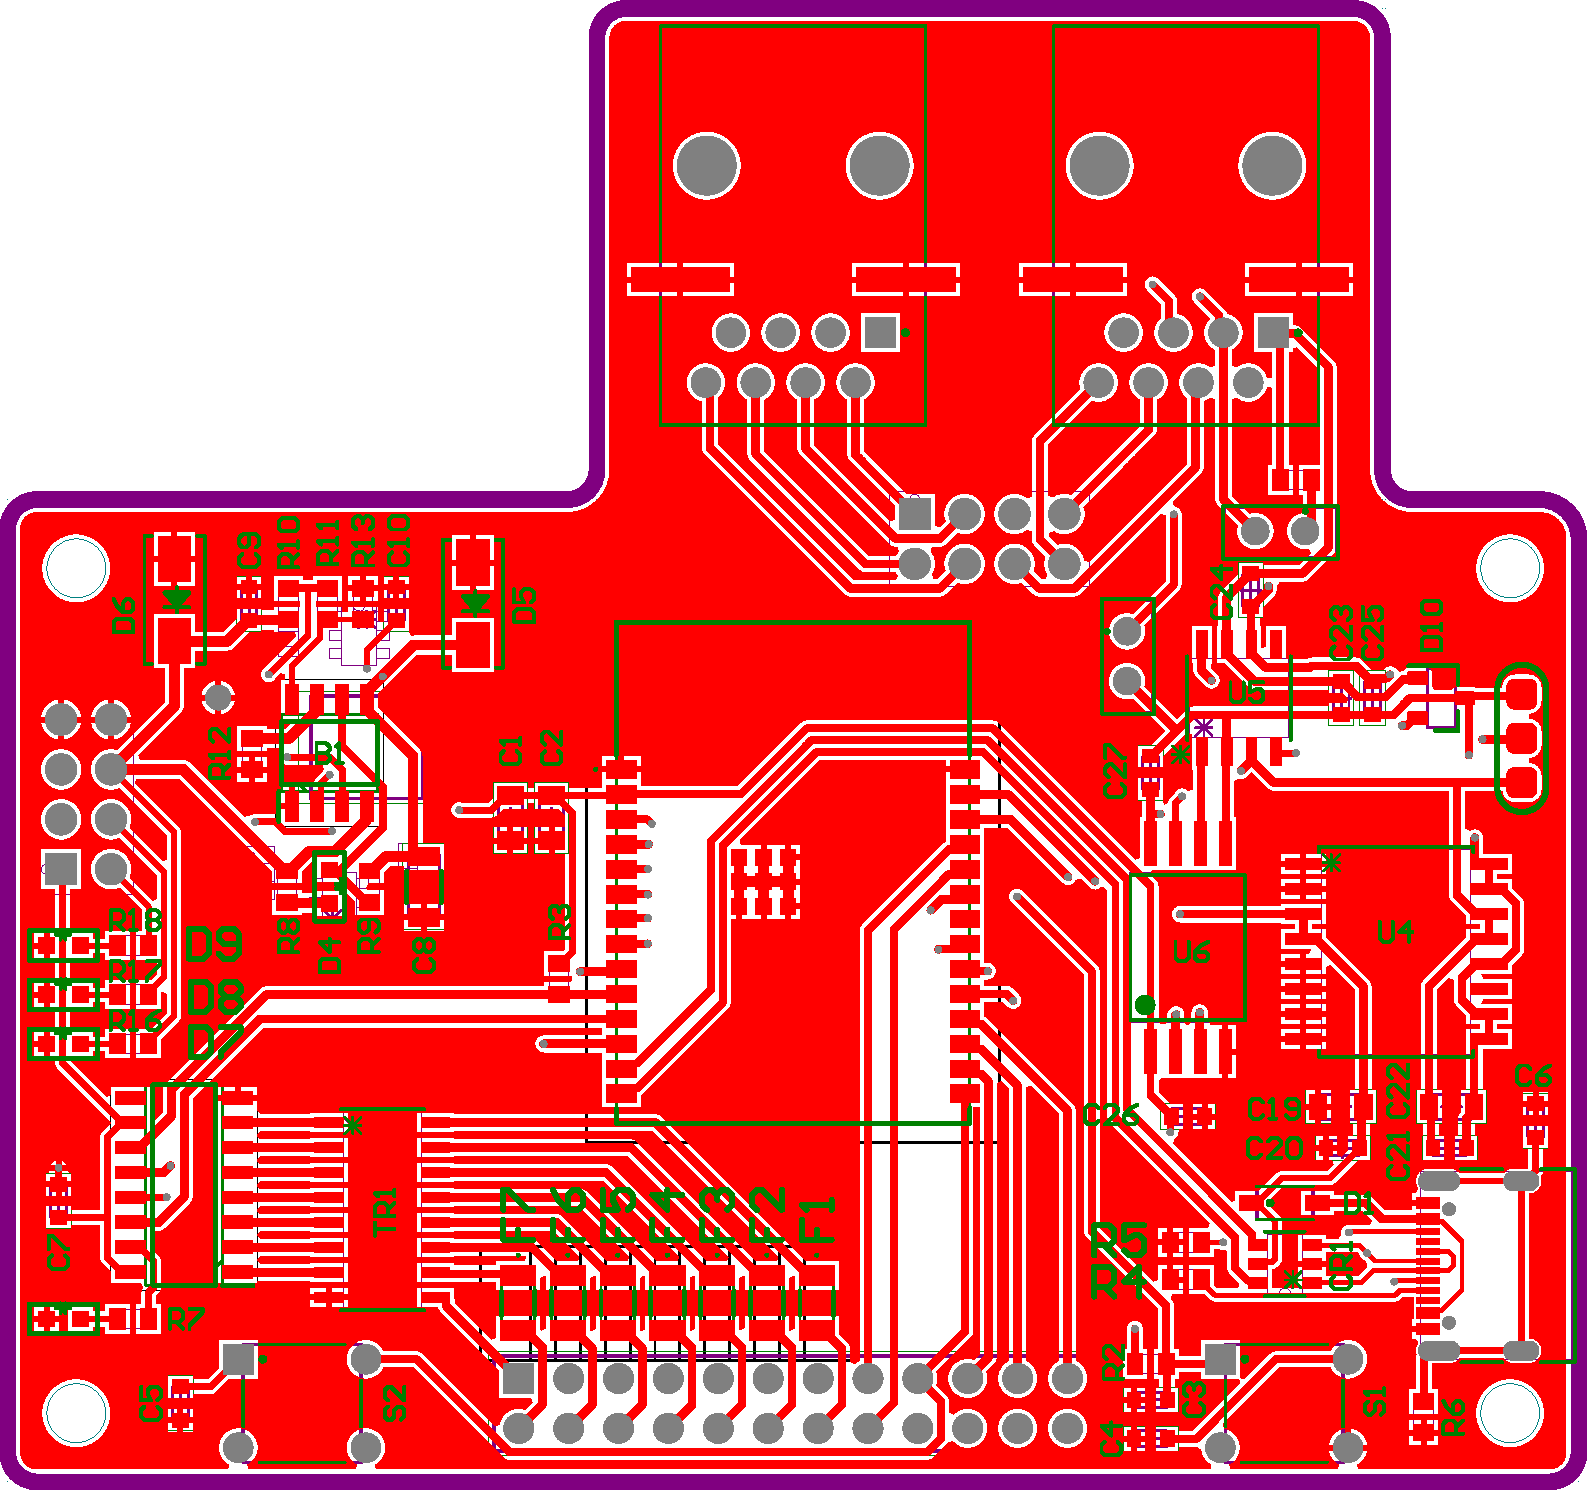
\includegraphics[width=\textwidth, page=1]{images/Job1.PDF}
		\caption{Top Layer}
		\label{fig:pcb1}
	\end{minipage}
	\hfill
	\begin{minipage}{0.48\textwidth}
		\centering
		\includegraphics[width=\textwidth, page=2]{images/Job1.PDF}
		\caption{Bottom Layer}
		\label{fig:pcb2}
	\end{minipage}
\end{figure}

A fentebbi ábrákon látható a korábbi schematicnak a nyákterve. Bal oldalon a felső oldal, jobb oldalon pedig az alsó oldal látható. Eredetileg szóba került, hogy a PCB 4, vagy akár 6 rétegő legyen, viszont végül mégis mardt 2 rétegű. Ennek számunkra több előnye is van. Mind amellett, hogy a gyártási költség a töredéke, így amennyiben a debuggolás közben kiderül, hogy valami félre lett kötve, felszínesen javítható. Amennyiben lennének belső rétegek, úgy ez már nem lenne kivitelezhető. Ami miatt még szintén teljesen megfelel számunkra a kettő rétegű konstrukció az az, hogy hellyel bőven gazdálkodhatunk, nem kell minden alkatrészt maximálisan összesűríteni, ezen felül azért sem lehet nagyon sűríteni, mert a kézi beültetés miatt helyet kell hagyni a pákahegynek, hogy beférjen a különböző alkatrészek közé.

Maga a PCB úgy lett megtervezve, hogy e mellé még illeszthető egy második kártya, ami a board különböző tüskesorain keresztül csatlakozik. Azért döntöttünk emellett a design mellett, mert így sokkal modulárisabb tud lenni az egész rendszer. Mindig a megfelelő alkalmazáshoz passzoló breakout-boardod lehet az aljára illesztneni, így el lehet kerülni a fölösleges sorkapcsokat, valamint méretben is kisebb tud maradni a teljes node.